\documentclass[11pt,a4paper,oneside]{article}
\usepackage[margin=15mm]{geometry}
\usepackage[ngerman]{babel}
\usepackage[hidelinks]{hyperref}
\usepackage{xcolor}
\usepackage{graphics}
\usepackage{tikz}
\usepackage{parskip}

\usetikzlibrary{arrows.meta}
\renewcommand{\familydefault}{\sfdefault}
\newcommand{\https}[1]{\href{https://#1}{\nolinkurl{#1}}}
\newcommand{\mailto}[1]{\href{mailto://#1}{\nolinkurl{#1}}}
\newcommand{\follownote}[1]{--- {\footnotesize\color{violet}#1}}
\newcommand{\prog}{Programmiersprache:}
\newcommand{\os}{Betriebssystem:}
\newcommand{\vcs}{Versionskontrollen:}
\newcommand{\issue}{Problemverfolgung:}
\newcommand{\acmicpcnote}[2]{--- {\footnotesize\color{violet}%
\href{https://icpc.baylor.edu/regionals/finder/#1/standings}%
{#2}%
}}
\newcommand{\codejamnote}[2]{--- {\footnotesize\color{violet}%
\href{https://codingcompetitions.withgoogle.com/codejam/round/#1}%
{#2}%
}}
\renewcommand{\section}[1]{%
{\large\textbf{#1}}\\
\rule[9pt]{18cm}{.4pt}\vspace{-15pt}%
}
\newenvironment{mytable}{%
\begin{tabular}{@{}l@{\hspace{4mm}}l@{}}%
}{\end{tabular}}
\newcommand{\myitem}[2]{%
\parbox[t]{16mm}{#1}&\parbox[t]{16cm}{#2}\\%
}
\newenvironment{innertable}{%
\begin{tabular}{@{}l@{\hspace{5mm}}l@{}}%
}{\end{tabular}}
\newcommand{\inneritem}[2]{%
\parbox{35mm}{{\color{darkgray}#1}}&\parbox{12cm}{#2}\\%
}

\pagestyle{empty}

\begin{document}%
\begin{tikzpicture}%
\clip circle (2cm);%
\node[anchor=center] {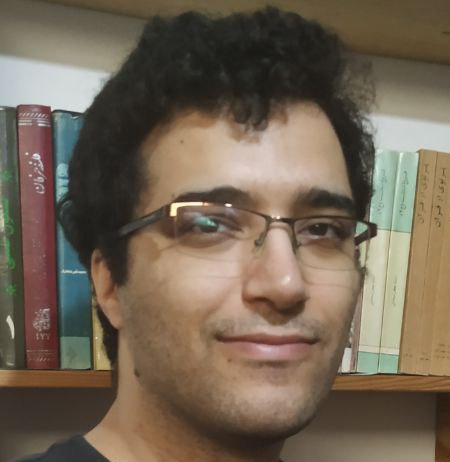
\includegraphics[width=4cm]{me}};%
\end{tikzpicture}%
\hspace{1cm}%
\parbox[b]{12cm}{%
\begin{tabbing}%
\hspace{3cm}\=\kill%
\textbf{{\LARGE Ali Farzanrad}}\\[5mm]
Geburtstag: \>
10{.} Mai, 1990\\[1mm]
E-Mail-Adresse: \>
\mailto{ali_farzanrad@riseup.net}\\[1mm]
GitHub: \>
\https{github.com/fmwviormv}\\[1mm]
LinkedIn: \>
\https{linkedin.com/in/ali-farzanrad-0635959b}\\[1mm]
Telefonnummer: \>
{+}98{ }911{ }871{ }3396\\
\end{tabbing}%
}

\section{Bildungsweg}

\begin{mytable}
\myitem{2012-09 -- 2015-02}{
\textbf{M.Sc.\ in Informatik}
\follownote{Technische Universit"at Amirkabir (Polytechnikum Teheran)}

\begin{innertable}
\inneritem{Hauptfach:}{Intelligente Systeme}
\inneritem{Gpa:}{15{,}07/20}
\inneritem{Abschlussarbeit:}{%
	"`Punkte mit Treppenpolygon abdecken"'}
\inneritem{Supervisor:}{Prof.~Ali~Mohades~Khorasani}
\end{innertable}
}
\end{mytable}

\begin{mytable}
\myitem{2008-09 -- 2012-09}{
\textbf{B.Sc.\ in Informatik}
\follownote{Technische Universit"at Amirkabir (Polytechnikum Teheran)}

\begin{innertable}
\inneritem{Gpa:}{15{,}80/20}
\inneritem{Abschlussarbeit:}{%
	Schnelle Polynomzeitreduktion zwischen vier verschiedenen
	Problemen bei bin"aren quadratischen Gleichungen}
\inneritem{Supervisor:}{Prof.~Mehdi~Ghatee}
\end{innertable}
}
\end{mytable}

\section{Berufserfahrung}

\begin{mytable}
\myitem{2020-05 -- current}{%
\textbf{Python Entwickler} bei
Mahsan Unternehmen, Teheran, Iran.

Entwicklung einer Befehlszeilenschnittstelle f"ur die Produkte
des Unternehmens,insbesondere f"ur die Firewall-Verwaltung.
Die Command Line ist verantwortlich f"ur die Interaktion mit dem Nutzer
"uber die System serielle Konsole und die entfernte ssh pty-Sitzung.
Die Benutzerbefehle variieren von Systemkonfiguration und Diagnose
zu Netzwerk-Dienstprogrammen mit Unterst"utzung
f"ur Autovervollst"andigung und intelligente Fehlerbehandlung
(mit benutzerfreundlichen Meldungen)

\begin{innertable}
\inneritem{\prog}{Python 3}
\inneritem{\os}{Ubuntu}
\inneritem{\vcs}{Git}
\inneritem{\issue}{Gitlab}
\end{innertable}
}
\end{mytable}

\begin{mytable}
\myitem{2019-03 -- 2020-04}{%
\textbf{Entwickler} bei
JAM Persia Unternehmen, Teheran, Iran.

Entwicklung eines Produktplanungs-Algorithmus f"ur das ERP-System
des Unternehmens.
Der Algorithmus ist zust"andig f"ur die Suche nach der bestm"oglichen
Auswahl und der Ressourcen zu finden, um die ben"otigten Produkte
p"unktlich zu produzieren.

\begin{innertable}
\inneritem{\prog}{C\#}
\inneritem{\os}{Windows}
\inneritem{\vcs}{SVN}
\inneritem{\issue}{Jira}
\end{innertable}
}
\end{mytable}

\begin{mytable}
\myitem{2017-01 -- 2018-06}{
\textbf{Entwickler} bei
Maharan Internationales Unternehmen, Teheran, Iran.

Entwicklung eines Zugsicherungssystems auf der Grundlage
der ERTMS-Spezifikationen.
Wir haben Hauptfunktionen f"ur die Verarbeitung und "Ubertragung
von High-Level-Signalen entwickelt.

\begin{innertable}
\inneritem{\prog}{C mit Frama-C}
\inneritem{\os}{Windows}
\inneritem{\vcs}{TFS}
\inneritem{\issue}{Microsoft Project}
\end{innertable}
}
\end{mytable}

\begin{mytable}
\myitem{2012-08 -- 2016-06}{
\textbf{Entwickler} bei
Negasht Unternehmen, Teheran, Iran.

Entwicklung webbasierter Anwendungen mit Karten und POI-Daten.

Entwicklung von Web-Services zur Erstellung von Kartenkacheln

Entwicklung von Web-Services zur Erstellung statischer Karten
aus Vektoren.

Entwicklung von Web-Services f"ur die Suche von k"urzesten Wegen
durch Angabe eines einfaches Paar von Breiten- und L"angengraden.

Die Entwicklung einer Android-App mit vielen verschiedenen
Umfrageformularen.

\begin{innertable}
\inneritem{\prog}{C\#, JavaScript, C++, und Java}
\inneritem{\os}{Windows}
\inneritem{\vcs}{Microsoft Visual SourceSafe}
\inneritem{\issue}{Unternehmensspezifische Fehlerverfolgung}
\end{innertable}
}
\end{mytable}

\section{Akademische Erfahrung}

\begin{mytable}\myitem{2017}{
Problem Designer und Test Designer f"ur den Vorregionalen ACM-ICPC
Programmier-Wettbewerb
\follownote{Technische Universit"at Amirkabir (Polytechnikum Teheran)}
}\end{mytable}

\begin{mytable}\myitem{2015}{
Teilnehmer der
\href{http://wscg.aut.ac.ir}{7{.} Winterschule f"ur Computergeometrie}
\follownote{Technische Universit"at Amirkabir (Polytechnikum Teheran)}
}\end{mytable}

\begin{mytable}\myitem{2013}{
Lehrassistent f"ur Betriebssysteme
\follownote{Technische Universit"at Amirkabir (Polytechnikum Teheran)}
}\end{mytable}

\section{Auszeichnungen}

\begin{mytable}\myitem{2017}{
Platz 474{.} unter mehr als 25{.}000 Teilnehmer
\codejamnote{0000000000201900}{Google CodeJam Round 2}
}\end{mytable}

\begin{mytable}\myitem{2015}{
Platz 2{.} in der Ph.D.-Eingangspr"ufung
\follownote{Nationale Universit"atsaufnahmepr"ufung}
}\end{mytable}

\begin{mytable}\myitem{2013}{
Platz 2{.} unter allen nationalen Universit"aten
\acmicpcnote{Tehran-2013}{ACM-ICPC Asien Teheran Regionalwettbewerb}
}\end{mytable}

\begin{mytable}\myitem{2013}{
Platz 67{.} unter "uber 2{.}000 Universit"aten
\follownote{Die 37{.} ACM-ICPC Weltmeisterschaft}
}\end{mytable}

\begin{mytable}\myitem{2012}{
Platz 1{.} unter 66 Mannschaften
\acmicpcnote{Kanpur-2012}
{ACM-ICPC Asia Kanpur Regionalwettbewerb}
}\end{mytable}

\begin{mytable}\myitem{2012}{
Platz 6{.} in der M.Sc.-Eingangspr"ufung
\follownote{Nationale Universit"atsaufnahmepr"ufung}
}\end{mytable}

\begin{mytable}\myitem{2011}{
Platz 4{.} unter 76 Mannschaften
\acmicpcnote{Tehran-2011}
{ACM-ICPC Asien Teheran Regionalwettbewerb}
}\end{mytable}

\begin{mytable}\myitem{2007}{
Silbermedaille bei der Nationalen Informatik-Olympiade
}\end{mytable}

\section{Interessen}
\begin{itemize}
\item Niedere Programmiersprache (C, Socketprogrammierung, libevent)
\item Nebenl"aufigkeit (Ereignisorientierte Programmierung,
	Multithreading, Monitoren/Semaphoren)
\item Algorithmen (Graph, Geometrie, Compiler)
\end{itemize}

\section{F"ahigkeiten und Kenntnisse}
\begin{itemize}
\item C (C89/90, C99, C11, libevent, pthreads, yacc, lex)
\item Python (Python 3.x, async)
\item C++ (C++98, C++11, C++14)
\item Java (Java 7, Java 8)
\item C\# (.Net Framework 4.x, ASP.NET MVC, .Net Core 2.x \& 3.x)
\item JavaScript (ES5.x, ES6)
\item Assembly (6502, 8086, i386, amd64, intel/at\&t syntax, SIMD)
\item UNIX Shell (sh, ksh, bash, sed, awk)
\end{itemize}

\section{Sprachkenntnisse}

\begin{mytable}\myitem{Englisch}{
	B2, TOEFL 79
}\end{mytable}

\begin{mytable}\myitem{Deutsch}{
	A1
}\end{mytable}

\end{document}
